\section{Introducción}

El propósito del presente informe es entregar una guía de apoyo para comprender como se realizó la modificación del montaje del motor de corriente continua. Anteriormente este contaba solamente con un motor de corriente continua y la única variable medida era la velocidad rotacional del eje del motor. Dada la necesidad de implementar un sistema de lazos anidados y además de aplicar una carga mecánica que ejerza torque al motor eléctrico, se implementó un sistema de medición de corriente para poder comunicar la corriente de armadura que consume el motor DC con el programa que realiza el control, se acopló mecánicamente un generador eléctrico, y, además, se implementó un módulo de carga electrónica conectada a la armadura del generador que permite ser controlado desde el computador para aumentar o disminuir la carga del generador.\\

En las siguientes secciones se deescribirá en detalle como se conforma el sistema completo, tanto a nivel físico como computacional, y también, como se implementaron todas las adiciones.\\

\section{Setup físico}

A continuación, se presenta una descripción general de la conexión entre los módulos del setup, utilizando diagramas de bloques como apoyo.

\subsection{Descripción del setup físico}

El setup físico consta de un motor eléctrico acoplado mecánicamente a un generador eléctrico. Ambos son máquinas de corriente continua con dos terminales para la excitación de campo y dos terminales para el acceso a la armadura. Para controlar el motor eléctrico, se utiliza un computador con sistema operativo Windows y el software Simulink, perteneciente a la familia de MATLAB. Este software permite implementar las estrategias de control aplicadas a las máquinas.

La comunicación entre el computador y el sistema físico se realiza mediante un módulo comercial OPTO-22. Este módulo establece una comunicación por protocolo Ethernet, formando una red directa entre el computador y el OPTO-22 mediante un cable Ethernet. La Figura \ref{fig:esquema} muestra un diagrama global del setup.

\begin{figure}[H]
    \centering
    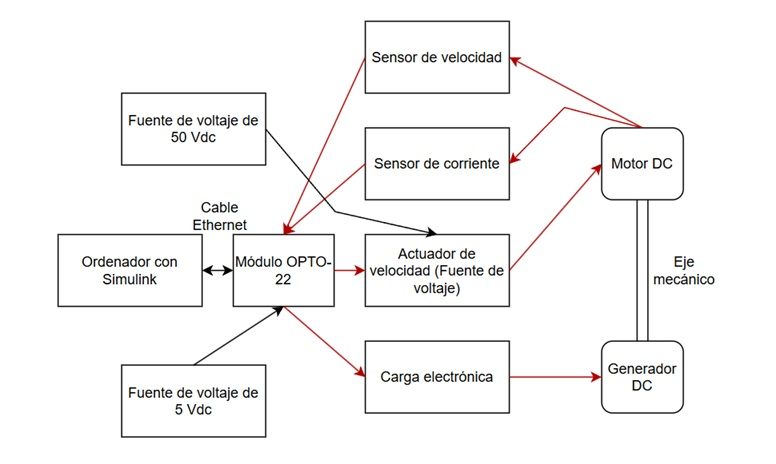
\includegraphics[width=0.75\linewidth]{img/diagramaGlobal.jpg}
    \caption{Esquema completo del sistema}
    \label{fig:esquema}
\end{figure}

\subsection{Componentes del setup}

El sistema implementado está compuesto por distintos módulos electrónicos y computacionales que permiten realizar el control, la adquisición de datos y la aplicación de carga sobre la máquina de corriente continua. Cada componente cumple una función específica dentro del lazo de control y adquisición del sistema. A continuación, se describe el propósito y funcionamiento general de cada uno de ellos.

\subsubsection{Módulo OPTO-22}

El módulo OPTO-22 corresponde a la interfaz principal entre el computador y el sistema físico. 
Este dispositivo permite adquirir señales analógicas provenientes de sensores y, además, 
generar señales analógicas de control hacia los actuadores del sistema. Para realizar su funcion, requiere de una alimentacion de 5 Vdc.\\

La comunicación entre el computador y el módulo OPTO-22 (ver Figura \ref{fig:OPTO22}) se realiza mediante protocolo Ethernet, 
estableciendo una red directa entre ambos dispositivos. Desde Simulink se envían comandos de voltaje hacia el motor y la carga electrónica, 
mientras que el OPTO-22 retorna las mediciones de velocidad y corriente para ser utilizadas posteriormentepor los algoritmos de control.

\begin{figure}[H]
    \centering
    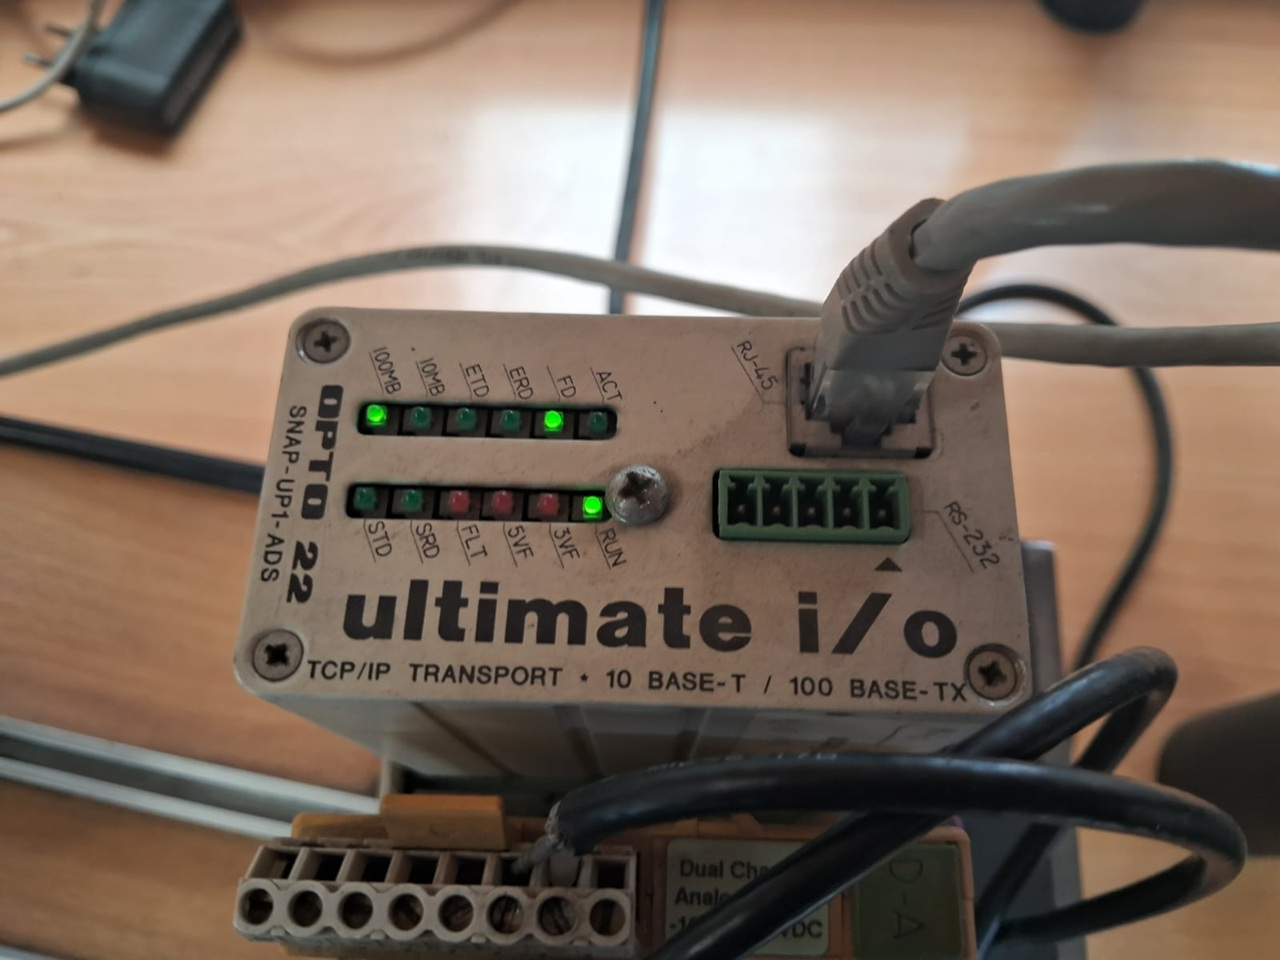
\includegraphics[width=0.75\linewidth]{img/OPTO22.jpg}
    \caption{Vista del OPTO22}
    \label{fig:OPTO22}
\end{figure}


En la implementación actual se utilizan los módulos SNAP-AOV-27 para las salidas analógicas y SNAP-AIV-4 para las entradas analógicas (ver Figura \ref{fig:snap}. Los rangos de voltaje que soportan ambos modulos son de -10 a 10 V de forma continua.


\begin{figure}[H]
    \centering
    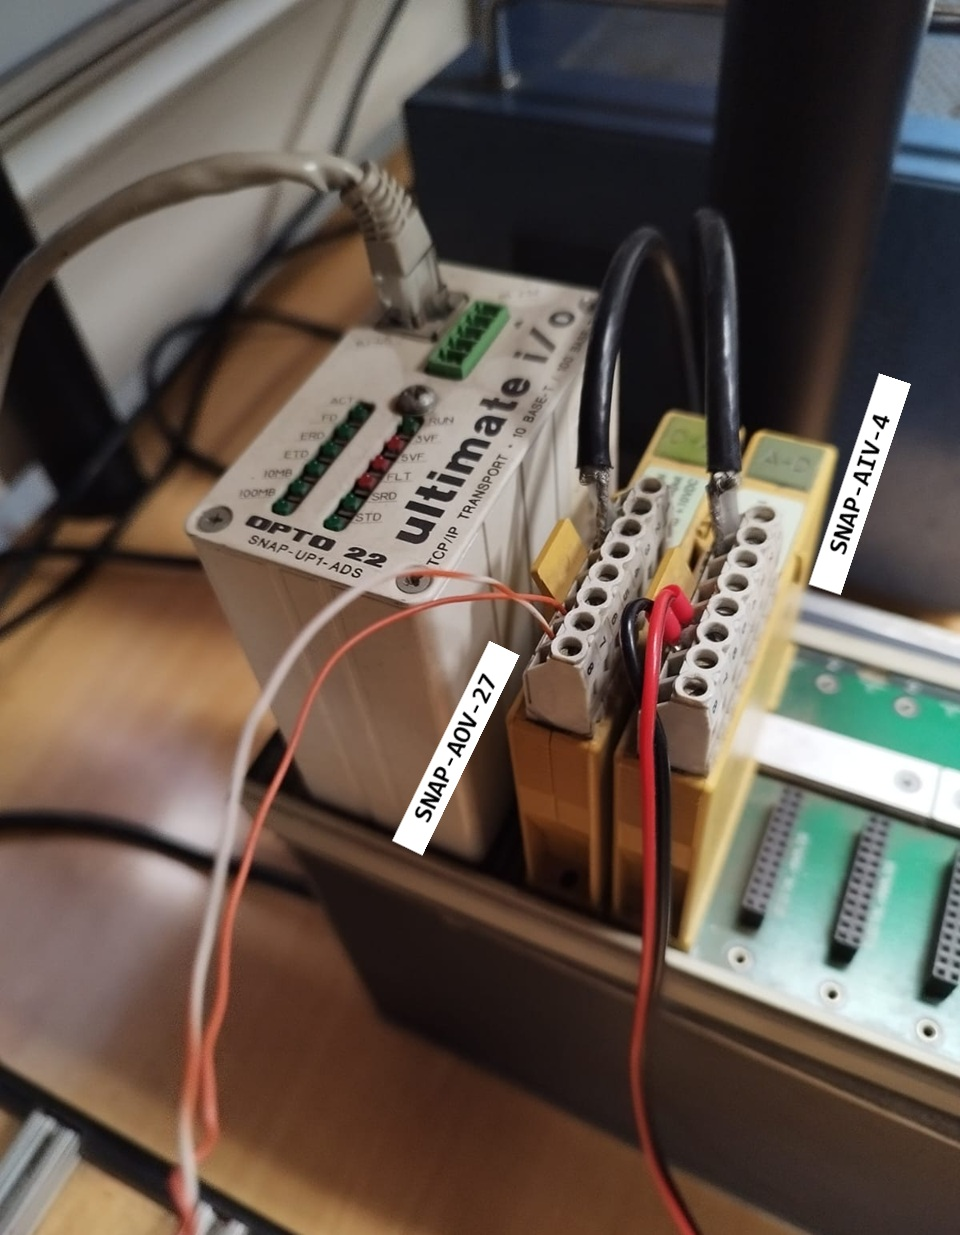
\includegraphics[width=0.75\linewidth]{img/snap.jpg}
    \caption{Vista de los modulos de entradas y salidas analogicas SNAP-AIV-4 y SNAP-AOV-27 respectivamente}
    \label{fig:snap}
\end{figure}

NOTA: La alimentacion de 5 Vdc necesaria para alimentar el modulo OPTO-22 proviene del Actuador de velocidad.

\subsubsection{Actuador de velocidad}

El actuador de velocidad es el modulo mostrado en la siguiente Figura \ref{fig:ActV}. 

\begin{figure}[H]
    \centering

    \subfloat[Primera imagen.\label{fig:ActV1}]{
        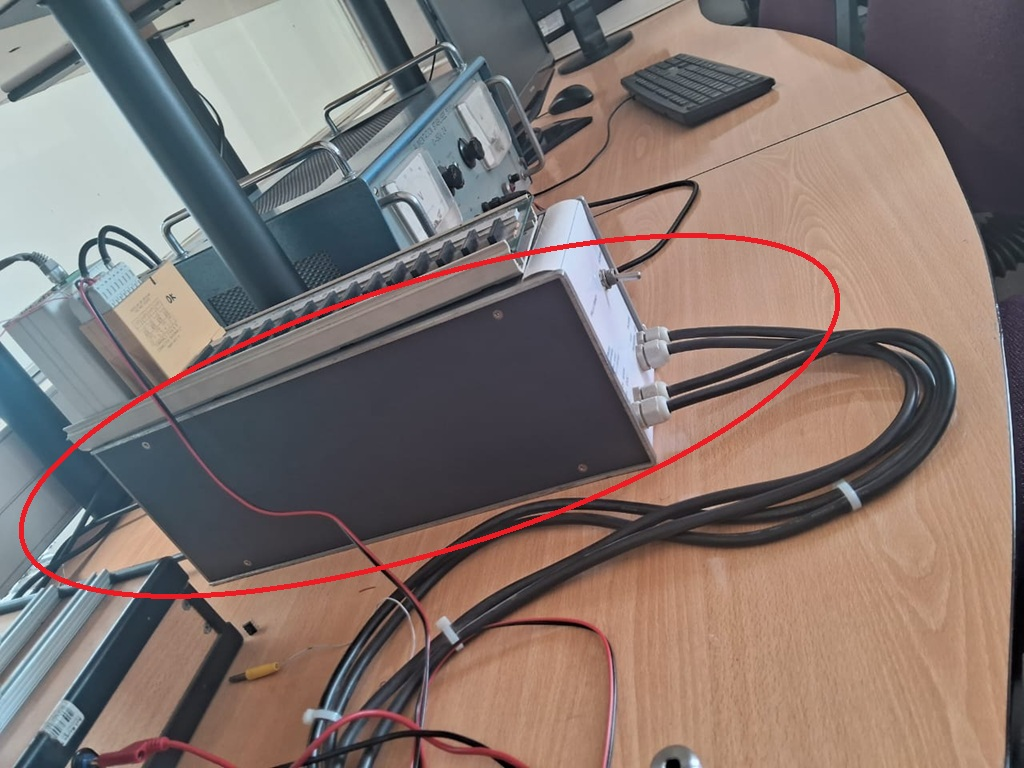
\includegraphics[width=0.5\textwidth]{img/ActV1.jpg}
    }
    \hfill
    \subfloat[Segunda imagen.\label{fig:ActV2}]{
        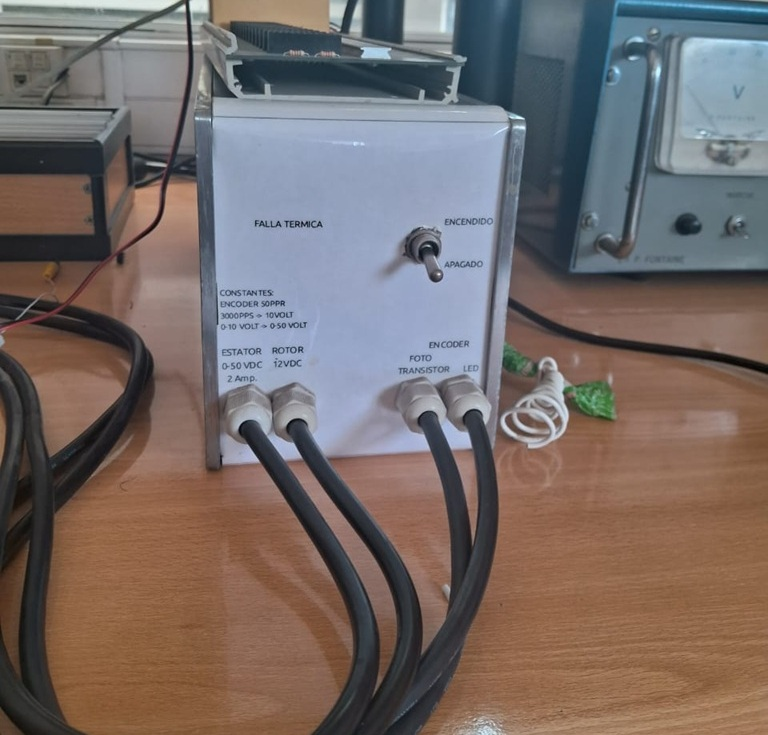
\includegraphics[width=0.5\textwidth]{img/ActV2.jpg}
    }

    \caption{Comparación entre ambas imágenes.}
    \label{fig:ActV}
\end{figure}

Dicho modulo recibe la señal de velocidad enviada desde Simulink mediante OPTO-22 a través del módulo de salidas analógicas SNAP-AOV-27, y, le aplica una amplificación de voltaje de un factor de aproximadamente 4, además, le agrega una etapa de potencia a la señal para ser aplicada a los bornes de la armadura del motor (lo cuál demanda un consumo de corriente). El funcionamiento interno del actuador se desconoce, pero se presume que puede ser un amplificador de voltaje seguido un amplificador de corriente para otorgar potencia al motor.

NOTA: Este modulo se alimenta mediante una fuente de 50 Vdc.

\subsubsection{Sensor de velocidad}

La velocidad angular del motor se mide mediante un sensor de velocidad basado en un disco con agujeros acoplado al eje del motor y un foto transistor acoplado opticamente con un diodo led infrarrojo los cuales al quedar alineados con un agujero del disco activan un 1 logico, lo que genera una señal con cierta frecuencia que permite determinar la velocidad rotacional del motor. Ver Figura \ref{fig:Encoder}.

\begin{figure}[H]
    \centering
    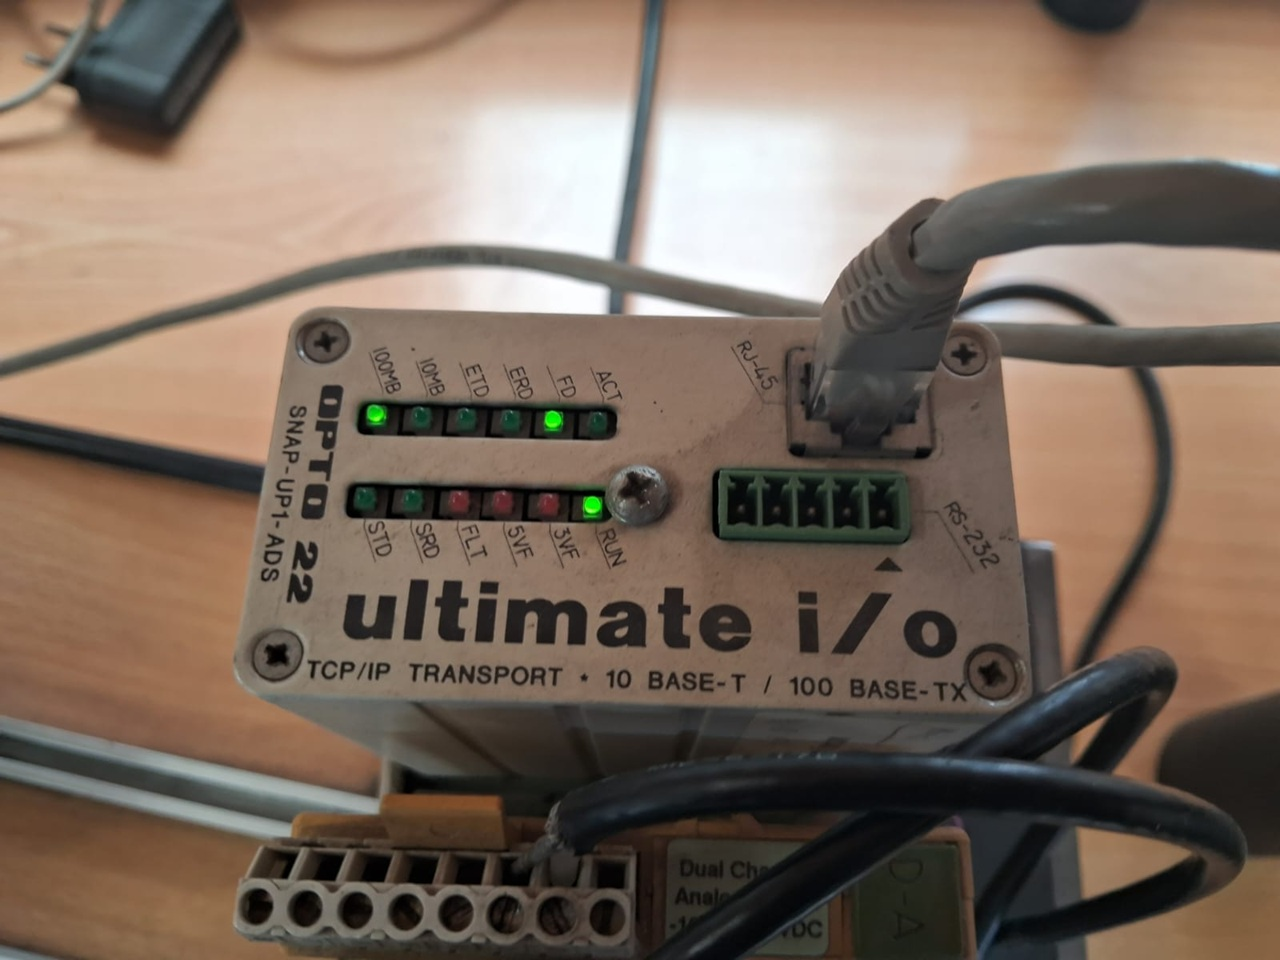
\includegraphics[width=0.75\linewidth]{img/Encoder.jpg}
    \caption{Vista del Encoder}
    \label{fig:Encoder}
\end{figure}

Dicha señal pulsante se envía al módulo que contiene al actuador de velocidad (ver Figura \ref{fig:ActV}), para ser transformada a un voltaje proporcional a la velocidad rotacional del eje mecánico del motor. Esta señal continua es enviada al módulo OPTO-22 mediante el módulo de entradas analógicas SNAP-AIV-4 para ser digitalizada y procesada en Simulink.

NOTA: La cantidad de agujeros que posee el disco se desconoce, pues no es necesario ya que dicha labor se encuentra correctamente implementada. 

\subsubsection{Sensor de corriente}

Con el fin de medir la corriente de armadura consumida por el motor, se implementó una PCB dedicada (más detalles en la seccion 'Solucion') basada en el sensor LA 55-P. 
Este sensor permite realizar mediciones de corriente con aislamiento eléctrico y sin intervenir directamente el circuito de potencia.

La señal entregada por el sensor es acondicionada mediante amplificadores operacionales y circuitos limitadores para obtener un rango compatible con las entradas analógicas del OPTO-22. Por último, al igual que el sensor de velocidad, la señal de corriente es entregada como voltaje analógico al módulo SNAP-AIV-4. \\

Nota: El módulo de medición de corriente también puede utilizarse para otros tipos de mediciones, por ejemplo, la corriente de campo del motor.

\subsubsection{Carga electrónica}
La carga electrónica fue diseñada con el propósito de aplicar una carga variable sobre el generador DC acoplado mecánicamente al motor  (más detalles en la seccion 'Solucion'). 
Esto permite simular distintas condiciones de carga y evaluar el comportamiento dinámico del sistema bajo diferentes exigencias. \\

La carga es controlada mediante una señal analógica proveniente del OPTO-22 (salida desde el módulo SNAP-AOV-27), permitiendo variar la corriente consumida por el circuito de potencia.
Internamente, la etapa de disipación utiliza un transistor TIP41C montado sobre un disipador térmico.

